% !TEX encoding = UTF-8 Unicode
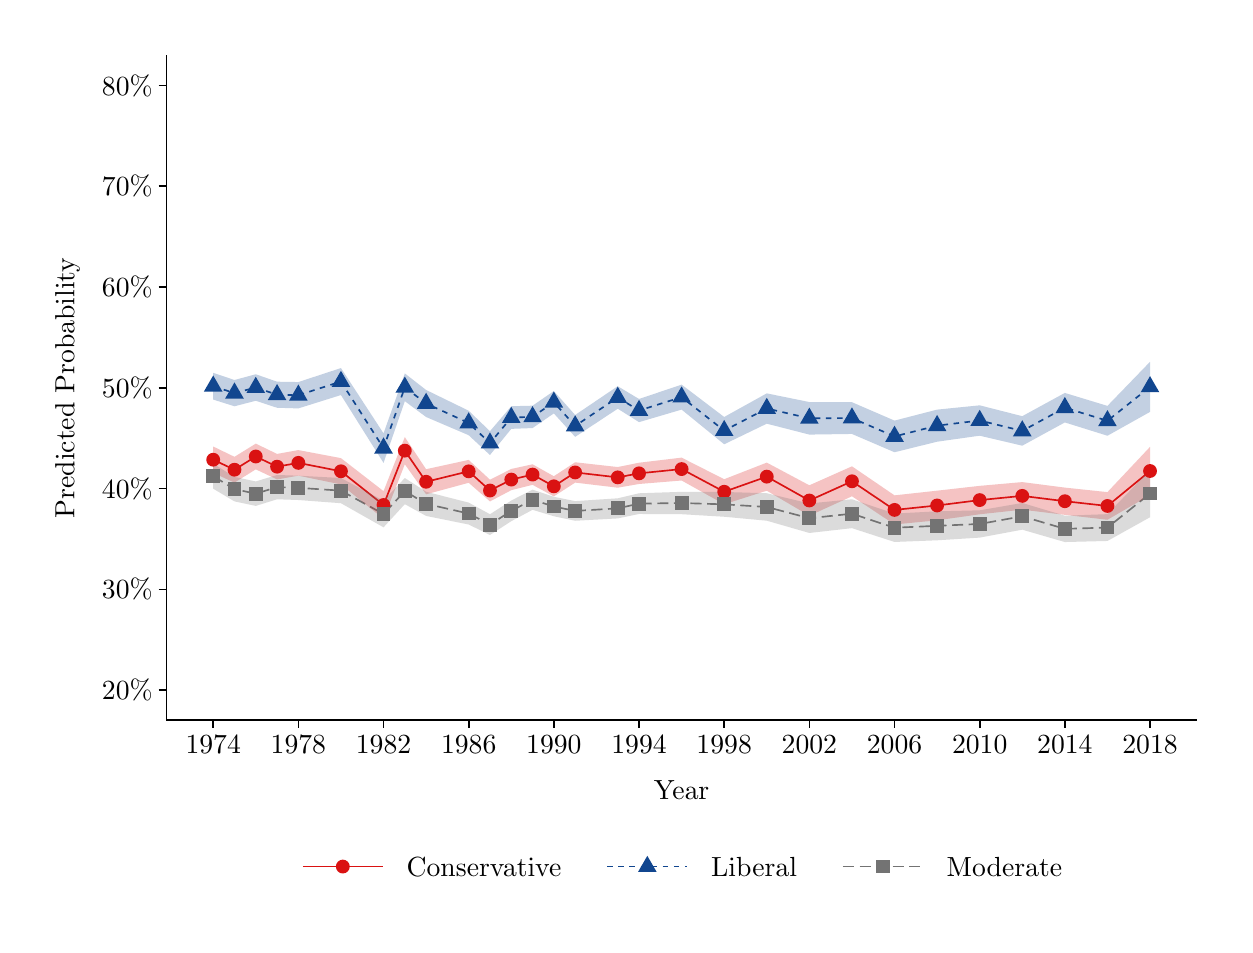
\begin{tikzpicture}[x=1pt,y=1pt]
\definecolor{fillColor}{RGB}{255,255,255}
\path[use as bounding box,fill=fillColor,fill opacity=0.00] (0,0) rectangle (432.48,324.36);
\begin{scope}
\path[clip] (  0.00,  0.00) rectangle (432.48,324.36);
\definecolor{fillColor}{RGB}{255,255,255}

\path[fill=fillColor] ( -0.00,  0.00) rectangle (432.48,324.36);
\end{scope}
\begin{scope}
\path[clip] ( 50.11, 74.07) rectangle (422.48,314.36);
\definecolor{fillColor}{RGB}{255,255,255}

\path[fill=fillColor] ( 50.11, 74.07) rectangle (422.48,314.36);
\definecolor{drawColor}{RGB}{218,18,18}

\path[draw=drawColor,line width= 0.6pt,line join=round] ( 67.04,168.24) --
	( 74.73,164.62) --
	( 82.42,169.40) --
	( 90.12,165.72) --
	( 97.81,167.10) --
	(113.20,164.06) --
	(128.59,151.88) --
	(136.28,171.51) --
	(143.97,160.27) --
	(159.36,164.04) --
	(167.05,157.10) --
	(174.75,161.06) --
	(182.44,162.87) --
	(190.13,158.62) --
	(197.83,163.64) --
	(213.22,161.86) --
	(220.91,163.31) --
	(236.30,164.86) --
	(251.68,156.66) --
	(267.07,162.12) --
	(282.46,153.50) --
	(297.85,160.44) --
	(313.23,150.10) --
	(328.62,151.70) --
	(344.01,153.65) --
	(359.39,155.17) --
	(374.78,153.24) --
	(390.17,151.53) --
	(405.56,164.16);
\definecolor{drawColor}{RGB}{17,70,143}

\path[draw=drawColor,line width= 0.6pt,dash pattern=on 2pt off 2pt ,line join=round] ( 67.04,194.80) --
	( 74.73,192.30) --
	( 82.42,194.33) --
	( 90.12,191.72) --
	( 97.81,191.54) --
	(113.20,196.49) --
	(128.59,172.43) --
	(136.28,194.41) --
	(143.97,188.56) --
	(159.36,181.51) --
	(167.05,174.24) --
	(174.75,183.48) --
	(182.44,183.72) --
	(190.13,189.01) --
	(197.83,180.45) --
	(213.22,190.74) --
	(220.91,186.01) --
	(236.30,190.86) --
	(251.68,178.75) --
	(267.07,186.74) --
	(282.46,183.20) --
	(297.85,183.28) --
	(313.23,176.65) --
	(328.62,180.55) --
	(344.01,182.41) --
	(359.39,178.64) --
	(374.78,187.04) --
	(390.17,182.30) --
	(405.56,194.56);
\definecolor{drawColor}{gray}{0.45}

\path[draw=drawColor,line width= 0.6pt,dash pattern=on 4pt off 2pt ,line join=round] ( 67.04,162.29) --
	( 74.73,157.61) --
	( 82.42,155.97) --
	( 90.12,158.33) --
	( 97.81,158.08) --
	(113.20,157.07) --
	(128.59,148.61) --
	(136.28,156.91) --
	(143.97,152.29) --
	(159.36,148.78) --
	(167.05,144.79) --
	(174.75,149.76) --
	(182.44,153.78) --
	(190.13,151.33) --
	(197.83,149.73) --
	(213.22,150.66) --
	(220.91,152.37) --
	(236.30,152.59) --
	(251.68,152.11) --
	(267.07,151.16) --
	(282.46,147.10) --
	(297.85,148.73) --
	(313.23,143.65) --
	(328.62,144.36) --
	(344.01,145.02) --
	(359.39,147.79) --
	(374.78,143.25) --
	(390.17,143.72) --
	(405.56,156.01);
\definecolor{fillColor}{RGB}{218,18,18}

\path[fill=fillColor,fill opacity=0.25] ( 67.04,173.01) --
	( 74.73,169.28) --
	( 82.42,174.05) --
	( 90.12,170.33) --
	( 97.81,171.72) --
	(113.20,168.81) --
	(128.59,156.88) --
	(136.28,176.41) --
	(143.97,164.81) --
	(159.36,168.16) --
	(167.05,161.02) --
	(174.75,164.90) --
	(182.44,166.58) --
	(190.13,162.27) --
	(197.83,167.31) --
	(213.22,165.59) --
	(220.91,167.15) --
	(236.30,168.99) --
	(251.68,161.19) --
	(267.07,167.19) --
	(282.46,158.99) --
	(297.85,165.85) --
	(313.23,155.36) --
	(328.62,157.05) --
	(344.01,158.79) --
	(359.39,160.15) --
	(374.78,158.16) --
	(390.17,156.53) --
	(405.56,172.88) --
	(405.56,155.44) --
	(390.17,146.54) --
	(374.78,148.32) --
	(359.39,150.19) --
	(344.01,148.52) --
	(328.62,146.34) --
	(313.23,144.84) --
	(297.85,155.03) --
	(282.46,148.01) --
	(267.07,157.04) --
	(251.68,152.14) --
	(236.30,160.73) --
	(220.91,159.47) --
	(213.22,158.13) --
	(197.83,159.97) --
	(190.13,154.98) --
	(182.44,159.17) --
	(174.75,157.23) --
	(167.05,153.17) --
	(159.36,159.91) --
	(143.97,155.73) --
	(136.28,166.60) --
	(128.59,146.87) --
	(113.20,159.31) --
	( 97.81,162.47) --
	( 90.12,161.11) --
	( 82.42,164.76) --
	( 74.73,159.96) --
	( 67.04,163.47) --
	cycle;

\path[] ( 67.04,173.01) --
	( 74.73,169.28) --
	( 82.42,174.05) --
	( 90.12,170.33) --
	( 97.81,171.72) --
	(113.20,168.81) --
	(128.59,156.88) --
	(136.28,176.41) --
	(143.97,164.81) --
	(159.36,168.16) --
	(167.05,161.02) --
	(174.75,164.90) --
	(182.44,166.58) --
	(190.13,162.27) --
	(197.83,167.31) --
	(213.22,165.59) --
	(220.91,167.15) --
	(236.30,168.99) --
	(251.68,161.19) --
	(267.07,167.19) --
	(282.46,158.99) --
	(297.85,165.85) --
	(313.23,155.36) --
	(328.62,157.05) --
	(344.01,158.79) --
	(359.39,160.15) --
	(374.78,158.16) --
	(390.17,156.53) --
	(405.56,172.88);

\path[] (405.56,155.44) --
	(390.17,146.54) --
	(374.78,148.32) --
	(359.39,150.19) --
	(344.01,148.52) --
	(328.62,146.34) --
	(313.23,144.84) --
	(297.85,155.03) --
	(282.46,148.01) --
	(267.07,157.04) --
	(251.68,152.14) --
	(236.30,160.73) --
	(220.91,159.47) --
	(213.22,158.13) --
	(197.83,159.97) --
	(190.13,154.98) --
	(182.44,159.17) --
	(174.75,157.23) --
	(167.05,153.17) --
	(159.36,159.91) --
	(143.97,155.73) --
	(136.28,166.60) --
	(128.59,146.87) --
	(113.20,159.31) --
	( 97.81,162.47) --
	( 90.12,161.11) --
	( 82.42,164.76) --
	( 74.73,159.96) --
	( 67.04,163.47);
\definecolor{fillColor}{RGB}{17,70,143}

\path[fill=fillColor,fill opacity=0.25] ( 67.04,199.63) --
	( 74.73,197.04) --
	( 82.42,199.12) --
	( 90.12,196.43) --
	( 97.81,196.30) --
	(113.20,201.36) --
	(128.59,177.76) --
	(136.28,199.42) --
	(143.97,193.44) --
	(159.36,185.94) --
	(167.05,178.54) --
	(174.75,187.57) --
	(182.44,187.76) --
	(190.13,193.05) --
	(197.83,184.40) --
	(213.22,194.80) --
	(220.91,190.19) --
	(236.30,195.37) --
	(251.68,183.68) --
	(267.07,192.21) --
	(282.46,189.08) --
	(297.85,189.02) --
	(313.23,182.37) --
	(328.62,186.34) --
	(344.01,187.89) --
	(359.39,183.97) --
	(374.78,192.37) --
	(390.17,187.69) --
	(405.56,203.61) --
	(405.56,185.52) --
	(390.17,176.90) --
	(374.78,181.71) --
	(359.39,173.31) --
	(344.01,176.92) --
	(328.62,174.75) --
	(313.23,170.94) --
	(297.85,177.55) --
	(282.46,177.32) --
	(267.07,181.26) --
	(251.68,173.82) --
	(236.30,186.35) --
	(220.91,181.82) --
	(213.22,186.67) --
	(197.83,176.49) --
	(190.13,184.97) --
	(182.44,179.68) --
	(174.75,179.39) --
	(167.05,169.95) --
	(159.36,177.09) --
	(143.97,183.68) --
	(136.28,189.39) --
	(128.59,167.09) --
	(113.20,191.61) --
	( 97.81,186.78) --
	( 90.12,187.01) --
	( 82.42,189.54) --
	( 74.73,187.55) --
	( 67.04,189.97) --
	cycle;

\path[] ( 67.04,199.63) --
	( 74.73,197.04) --
	( 82.42,199.12) --
	( 90.12,196.43) --
	( 97.81,196.30) --
	(113.20,201.36) --
	(128.59,177.76) --
	(136.28,199.42) --
	(143.97,193.44) --
	(159.36,185.94) --
	(167.05,178.54) --
	(174.75,187.57) --
	(182.44,187.76) --
	(190.13,193.05) --
	(197.83,184.40) --
	(213.22,194.80) --
	(220.91,190.19) --
	(236.30,195.37) --
	(251.68,183.68) --
	(267.07,192.21) --
	(282.46,189.08) --
	(297.85,189.02) --
	(313.23,182.37) --
	(328.62,186.34) --
	(344.01,187.89) --
	(359.39,183.97) --
	(374.78,192.37) --
	(390.17,187.69) --
	(405.56,203.61);

\path[] (405.56,185.52) --
	(390.17,176.90) --
	(374.78,181.71) --
	(359.39,173.31) --
	(344.01,176.92) --
	(328.62,174.75) --
	(313.23,170.94) --
	(297.85,177.55) --
	(282.46,177.32) --
	(267.07,181.26) --
	(251.68,173.82) --
	(236.30,186.35) --
	(220.91,181.82) --
	(213.22,186.67) --
	(197.83,176.49) --
	(190.13,184.97) --
	(182.44,179.68) --
	(174.75,179.39) --
	(167.05,169.95) --
	(159.36,177.09) --
	(143.97,183.68) --
	(136.28,189.39) --
	(128.59,167.09) --
	(113.20,191.61) --
	( 97.81,186.78) --
	( 90.12,187.01) --
	( 82.42,189.54) --
	( 74.73,187.55) --
	( 67.04,189.97);
\definecolor{fillColor}{RGB}{115,115,115}

\path[fill=fillColor,fill opacity=0.25] ( 67.04,166.82) --
	( 74.73,162.03) --
	( 82.42,160.39) --
	( 90.12,162.72) --
	( 97.81,162.47) --
	(113.20,161.62) --
	(128.59,153.41) --
	(136.28,161.63) --
	(143.97,156.66) --
	(159.36,152.74) --
	(167.05,148.54) --
	(174.75,153.49) --
	(182.44,157.42) --
	(190.13,154.84) --
	(197.83,153.28) --
	(213.22,154.29) --
	(220.91,156.11) --
	(236.30,156.63) --
	(251.68,156.59) --
	(267.07,156.12) --
	(282.46,152.43) --
	(297.85,153.94) --
	(313.23,148.78) --
	(328.62,149.59) --
	(344.01,149.95) --
	(359.39,152.61) --
	(374.78,148.00) --
	(390.17,148.57) --
	(405.56,164.56) --
	(405.56,147.45) --
	(390.17,138.88) --
	(374.78,138.49) --
	(359.39,142.96) --
	(344.01,140.09) --
	(328.62,139.12) --
	(313.23,138.52) --
	(297.85,143.51) --
	(282.46,141.77) --
	(267.07,146.20) --
	(251.68,147.63) --
	(236.30,148.55) --
	(220.91,148.63) --
	(213.22,147.03) --
	(197.83,146.18) --
	(190.13,147.81) --
	(182.44,150.14) --
	(174.75,146.03) --
	(167.05,141.04) --
	(159.36,144.82) --
	(143.97,147.93) --
	(136.28,152.18) --
	(128.59,143.81) --
	(113.20,152.52) --
	( 97.81,153.68) --
	( 90.12,153.94) --
	( 82.42,151.55) --
	( 74.73,153.18) --
	( 67.04,157.77) --
	cycle;

\path[] ( 67.04,166.82) --
	( 74.73,162.03) --
	( 82.42,160.39) --
	( 90.12,162.72) --
	( 97.81,162.47) --
	(113.20,161.62) --
	(128.59,153.41) --
	(136.28,161.63) --
	(143.97,156.66) --
	(159.36,152.74) --
	(167.05,148.54) --
	(174.75,153.49) --
	(182.44,157.42) --
	(190.13,154.84) --
	(197.83,153.28) --
	(213.22,154.29) --
	(220.91,156.11) --
	(236.30,156.63) --
	(251.68,156.59) --
	(267.07,156.12) --
	(282.46,152.43) --
	(297.85,153.94) --
	(313.23,148.78) --
	(328.62,149.59) --
	(344.01,149.95) --
	(359.39,152.61) --
	(374.78,148.00) --
	(390.17,148.57) --
	(405.56,164.56);

\path[] (405.56,147.45) --
	(390.17,138.88) --
	(374.78,138.49) --
	(359.39,142.96) --
	(344.01,140.09) --
	(328.62,139.12) --
	(313.23,138.52) --
	(297.85,143.51) --
	(282.46,141.77) --
	(267.07,146.20) --
	(251.68,147.63) --
	(236.30,148.55) --
	(220.91,148.63) --
	(213.22,147.03) --
	(197.83,146.18) --
	(190.13,147.81) --
	(182.44,150.14) --
	(174.75,146.03) --
	(167.05,141.04) --
	(159.36,144.82) --
	(143.97,147.93) --
	(136.28,152.18) --
	(128.59,143.81) --
	(113.20,152.52) --
	( 97.81,153.68) --
	( 90.12,153.94) --
	( 82.42,151.55) --
	( 74.73,153.18) --
	( 67.04,157.77);
\definecolor{fillColor}{RGB}{17,70,143}

\path[fill=fillColor] ( 67.04,198.68) --
	( 70.40,192.86) --
	( 63.67,192.86) --
	cycle;

\path[fill=fillColor] ( 74.73,196.18) --
	( 78.09,190.35) --
	( 71.37,190.35) --
	cycle;

\path[fill=fillColor] ( 82.42,198.21) --
	( 85.79,192.39) --
	( 79.06,192.39) --
	cycle;

\path[fill=fillColor] ( 90.12,195.60) --
	( 93.48,189.78) --
	( 86.75,189.78) --
	cycle;

\path[fill=fillColor] ( 97.81,195.42) --
	(101.17,189.60) --
	( 94.45,189.60) --
	cycle;

\path[fill=fillColor] (113.20,200.37) --
	(116.56,194.54) --
	(109.83,194.54) --
	cycle;

\path[fill=fillColor] (128.59,176.31) --
	(131.95,170.48) --
	(125.22,170.48) --
	cycle;

\path[fill=fillColor] (136.28,198.29) --
	(139.64,192.46) --
	(132.91,192.46) --
	cycle;

\path[fill=fillColor] (143.97,192.44) --
	(147.34,186.62) --
	(140.61,186.62) --
	cycle;

\path[fill=fillColor] (159.36,185.40) --
	(162.72,179.57) --
	(156.00,179.57) --
	cycle;

\path[fill=fillColor] (167.05,178.13) --
	(170.42,172.30) --
	(163.69,172.30) --
	cycle;

\path[fill=fillColor] (174.75,187.36) --
	(178.11,181.54) --
	(171.38,181.54) --
	cycle;

\path[fill=fillColor] (182.44,187.60) --
	(185.80,181.78) --
	(179.08,181.78) --
	cycle;

\path[fill=fillColor] (190.13,192.89) --
	(193.50,187.07) --
	(186.77,187.07) --
	cycle;

\path[fill=fillColor] (197.83,184.33) --
	(201.19,178.50) --
	(194.46,178.50) --
	cycle;

\path[fill=fillColor] (213.22,194.62) --
	(216.58,188.80) --
	(209.85,188.80) --
	cycle;

\path[fill=fillColor] (220.91,189.89) --
	(224.27,184.07) --
	(217.54,184.07) --
	cycle;

\path[fill=fillColor] (236.30,194.74) --
	(239.66,188.92) --
	(232.93,188.92) --
	cycle;

\path[fill=fillColor] (251.68,182.63) --
	(255.05,176.81) --
	(248.32,176.81) --
	cycle;

\path[fill=fillColor] (267.07,190.62) --
	(270.43,184.79) --
	(263.71,184.79) --
	cycle;

\path[fill=fillColor] (282.46,187.09) --
	(285.82,181.26) --
	(279.09,181.26) --
	cycle;

\path[fill=fillColor] (297.85,187.17) --
	(301.21,181.34) --
	(294.48,181.34) --
	cycle;

\path[fill=fillColor] (313.23,180.54) --
	(316.60,174.71) --
	(309.87,174.71) --
	cycle;

\path[fill=fillColor] (328.62,184.43) --
	(331.98,178.60) --
	(325.26,178.60) --
	cycle;

\path[fill=fillColor] (344.01,186.29) --
	(347.37,180.46) --
	(340.64,180.46) --
	cycle;

\path[fill=fillColor] (359.39,182.52) --
	(362.76,176.70) --
	(356.03,176.70) --
	cycle;

\path[fill=fillColor] (374.78,190.92) --
	(378.15,185.10) --
	(371.42,185.10) --
	cycle;

\path[fill=fillColor] (390.17,186.18) --
	(393.53,180.36) --
	(386.80,180.36) --
	cycle;

\path[fill=fillColor] (405.56,198.45) --
	(408.92,192.62) --
	(402.19,192.62) --
	cycle;
\definecolor{fillColor}{RGB}{218,18,18}

\path[fill=fillColor] ( 67.04,168.24) circle (  2.50);

\path[fill=fillColor] ( 74.73,164.62) circle (  2.50);

\path[fill=fillColor] ( 82.42,169.40) circle (  2.50);

\path[fill=fillColor] ( 90.12,165.72) circle (  2.50);

\path[fill=fillColor] ( 97.81,167.10) circle (  2.50);

\path[fill=fillColor] (113.20,164.06) circle (  2.50);

\path[fill=fillColor] (128.59,151.88) circle (  2.50);

\path[fill=fillColor] (136.28,171.51) circle (  2.50);

\path[fill=fillColor] (143.97,160.27) circle (  2.50);

\path[fill=fillColor] (159.36,164.04) circle (  2.50);

\path[fill=fillColor] (167.05,157.10) circle (  2.50);

\path[fill=fillColor] (174.75,161.06) circle (  2.50);

\path[fill=fillColor] (182.44,162.87) circle (  2.50);

\path[fill=fillColor] (190.13,158.62) circle (  2.50);

\path[fill=fillColor] (197.83,163.64) circle (  2.50);

\path[fill=fillColor] (213.22,161.86) circle (  2.50);

\path[fill=fillColor] (220.91,163.31) circle (  2.50);

\path[fill=fillColor] (236.30,164.86) circle (  2.50);

\path[fill=fillColor] (251.68,156.66) circle (  2.50);

\path[fill=fillColor] (267.07,162.12) circle (  2.50);

\path[fill=fillColor] (282.46,153.50) circle (  2.50);

\path[fill=fillColor] (297.85,160.44) circle (  2.50);

\path[fill=fillColor] (313.23,150.10) circle (  2.50);

\path[fill=fillColor] (328.62,151.70) circle (  2.50);

\path[fill=fillColor] (344.01,153.65) circle (  2.50);

\path[fill=fillColor] (359.39,155.17) circle (  2.50);

\path[fill=fillColor] (374.78,153.24) circle (  2.50);

\path[fill=fillColor] (390.17,151.53) circle (  2.50);

\path[fill=fillColor] (405.56,164.16) circle (  2.50);
\definecolor{fillColor}{gray}{0.45}

\path[fill=fillColor] ( 64.54,159.80) --
	( 69.53,159.80) --
	( 69.53,164.79) --
	( 64.54,164.79) --
	cycle;

\path[fill=fillColor] ( 72.23,155.11) --
	( 77.23,155.11) --
	( 77.23,160.10) --
	( 72.23,160.10) --
	cycle;

\path[fill=fillColor] ( 79.93,153.47) --
	( 84.92,153.47) --
	( 84.92,158.46) --
	( 79.93,158.46) --
	cycle;

\path[fill=fillColor] ( 87.62,155.84) --
	( 92.61,155.84) --
	( 92.61,160.83) --
	( 87.62,160.83) --
	cycle;

\path[fill=fillColor] ( 95.31,155.58) --
	(100.31,155.58) --
	(100.31,160.57) --
	( 95.31,160.57) --
	cycle;

\path[fill=fillColor] (110.70,154.57) --
	(115.70,154.57) --
	(115.70,159.56) --
	(110.70,159.56) --
	cycle;

\path[fill=fillColor] (126.09,146.11) --
	(131.08,146.11) --
	(131.08,151.11) --
	(126.09,151.11) --
	cycle;

\path[fill=fillColor] (133.78,154.41) --
	(138.78,154.41) --
	(138.78,159.40) --
	(133.78,159.40) --
	cycle;

\path[fill=fillColor] (141.47,149.80) --
	(146.47,149.80) --
	(146.47,154.79) --
	(141.47,154.79) --
	cycle;

\path[fill=fillColor] (156.86,146.28) --
	(161.86,146.28) --
	(161.86,151.27) --
	(156.86,151.27) --
	cycle;

\path[fill=fillColor] (164.56,142.29) --
	(169.55,142.29) --
	(169.55,147.29) --
	(164.56,147.29) --
	cycle;

\path[fill=fillColor] (172.25,147.26) --
	(177.24,147.26) --
	(177.24,152.25) --
	(172.25,152.25) --
	cycle;

\path[fill=fillColor] (179.94,151.28) --
	(184.94,151.28) --
	(184.94,156.28) --
	(179.94,156.28) --
	cycle;

\path[fill=fillColor] (187.64,148.83) --
	(192.63,148.83) --
	(192.63,153.82) --
	(187.64,153.82) --
	cycle;

\path[fill=fillColor] (195.33,147.23) --
	(200.33,147.23) --
	(200.33,152.23) --
	(195.33,152.23) --
	cycle;

\path[fill=fillColor] (210.72,148.16) --
	(215.71,148.16) --
	(215.71,153.16) --
	(210.72,153.16) --
	cycle;

\path[fill=fillColor] (218.41,149.87) --
	(223.41,149.87) --
	(223.41,154.87) --
	(218.41,154.87) --
	cycle;

\path[fill=fillColor] (233.80,150.09) --
	(238.79,150.09) --
	(238.79,155.09) --
	(233.80,155.09) --
	cycle;

\path[fill=fillColor] (249.19,149.62) --
	(254.18,149.62) --
	(254.18,154.61) --
	(249.19,154.61) --
	cycle;

\path[fill=fillColor] (264.57,148.66) --
	(269.57,148.66) --
	(269.57,153.66) --
	(264.57,153.66) --
	cycle;

\path[fill=fillColor] (279.96,144.60) --
	(284.96,144.60) --
	(284.96,149.60) --
	(279.96,149.60) --
	cycle;

\path[fill=fillColor] (295.35,146.23) --
	(300.34,146.23) --
	(300.34,151.22) --
	(295.35,151.22) --
	cycle;

\path[fill=fillColor] (310.73,141.15) --
	(315.73,141.15) --
	(315.73,146.15) --
	(310.73,146.15) --
	cycle;

\path[fill=fillColor] (326.12,141.86) --
	(331.12,141.86) --
	(331.12,146.85) --
	(326.12,146.85) --
	cycle;

\path[fill=fillColor] (341.51,142.52) --
	(346.50,142.52) --
	(346.50,147.52) --
	(341.51,147.52) --
	cycle;

\path[fill=fillColor] (356.90,145.29) --
	(361.89,145.29) --
	(361.89,150.28) --
	(356.90,150.28) --
	cycle;

\path[fill=fillColor] (372.28,140.75) --
	(377.28,140.75) --
	(377.28,145.74) --
	(372.28,145.74) --
	cycle;

\path[fill=fillColor] (387.67,141.23) --
	(392.67,141.23) --
	(392.67,146.22) --
	(387.67,146.22) --
	cycle;

\path[fill=fillColor] (403.06,153.51) --
	(408.05,153.51) --
	(408.05,158.50) --
	(403.06,158.50) --
	cycle;
\end{scope}
\begin{scope}
\path[clip] (  0.00,  0.00) rectangle (432.48,324.36);
\definecolor{drawColor}{RGB}{0,0,0}

\path[draw=drawColor,line width= 0.6pt,line join=round] ( 50.11, 74.07) --
	( 50.11,314.36);
\end{scope}
\begin{scope}
\path[clip] (  0.00,  0.00) rectangle (432.48,324.36);
\definecolor{drawColor}{RGB}{0,0,0}

\node[text=drawColor,anchor=base east,inner sep=0pt, outer sep=0pt, scale=  1.00] at ( 45.16, 81.55) {20{\%}};

\node[text=drawColor,anchor=base east,inner sep=0pt, outer sep=0pt, scale=  1.00] at ( 45.16,117.95) {30{\%}};

\node[text=drawColor,anchor=base east,inner sep=0pt, outer sep=0pt, scale=  1.00] at ( 45.16,154.36) {40{\%}};

\node[text=drawColor,anchor=base east,inner sep=0pt, outer sep=0pt, scale=  1.00] at ( 45.16,190.77) {50{\%}};

\node[text=drawColor,anchor=base east,inner sep=0pt, outer sep=0pt, scale=  1.00] at ( 45.16,227.18) {60{\%}};

\node[text=drawColor,anchor=base east,inner sep=0pt, outer sep=0pt, scale=  1.00] at ( 45.16,263.59) {70{\%}};

\node[text=drawColor,anchor=base east,inner sep=0pt, outer sep=0pt, scale=  1.00] at ( 45.16,300.00) {80{\%}};
\end{scope}
\begin{scope}
\path[clip] (  0.00,  0.00) rectangle (432.48,324.36);
\definecolor{drawColor}{RGB}{0,0,0}

\path[draw=drawColor,line width= 0.6pt,line join=round] ( 47.36, 84.99) --
	( 50.11, 84.99);

\path[draw=drawColor,line width= 0.6pt,line join=round] ( 47.36,121.40) --
	( 50.11,121.40);

\path[draw=drawColor,line width= 0.6pt,line join=round] ( 47.36,157.81) --
	( 50.11,157.81);

\path[draw=drawColor,line width= 0.6pt,line join=round] ( 47.36,194.21) --
	( 50.11,194.21);

\path[draw=drawColor,line width= 0.6pt,line join=round] ( 47.36,230.62) --
	( 50.11,230.62);

\path[draw=drawColor,line width= 0.6pt,line join=round] ( 47.36,267.03) --
	( 50.11,267.03);

\path[draw=drawColor,line width= 0.6pt,line join=round] ( 47.36,303.44) --
	( 50.11,303.44);
\end{scope}
\begin{scope}
\path[clip] (  0.00,  0.00) rectangle (432.48,324.36);
\definecolor{drawColor}{RGB}{0,0,0}

\path[draw=drawColor,line width= 0.6pt,line join=round] ( 50.11, 74.07) --
	(422.48, 74.07);
\end{scope}
\begin{scope}
\path[clip] (  0.00,  0.00) rectangle (432.48,324.36);
\definecolor{drawColor}{RGB}{0,0,0}

\path[draw=drawColor,line width= 0.6pt,line join=round] ( 67.04, 71.32) --
	( 67.04, 74.07);

\path[draw=drawColor,line width= 0.6pt,line join=round] ( 97.81, 71.32) --
	( 97.81, 74.07);

\path[draw=drawColor,line width= 0.6pt,line join=round] (128.59, 71.32) --
	(128.59, 74.07);

\path[draw=drawColor,line width= 0.6pt,line join=round] (159.36, 71.32) --
	(159.36, 74.07);

\path[draw=drawColor,line width= 0.6pt,line join=round] (190.13, 71.32) --
	(190.13, 74.07);

\path[draw=drawColor,line width= 0.6pt,line join=round] (220.91, 71.32) --
	(220.91, 74.07);

\path[draw=drawColor,line width= 0.6pt,line join=round] (251.68, 71.32) --
	(251.68, 74.07);

\path[draw=drawColor,line width= 0.6pt,line join=round] (282.46, 71.32) --
	(282.46, 74.07);

\path[draw=drawColor,line width= 0.6pt,line join=round] (313.23, 71.32) --
	(313.23, 74.07);

\path[draw=drawColor,line width= 0.6pt,line join=round] (344.01, 71.32) --
	(344.01, 74.07);

\path[draw=drawColor,line width= 0.6pt,line join=round] (374.78, 71.32) --
	(374.78, 74.07);

\path[draw=drawColor,line width= 0.6pt,line join=round] (405.56, 71.32) --
	(405.56, 74.07);
\end{scope}
\begin{scope}
\path[clip] (  0.00,  0.00) rectangle (432.48,324.36);
\definecolor{drawColor}{RGB}{0,0,0}

\node[text=drawColor,anchor=base,inner sep=0pt, outer sep=0pt, scale=  1.00] at ( 67.04, 62.23) {1974};

\node[text=drawColor,anchor=base,inner sep=0pt, outer sep=0pt, scale=  1.00] at ( 97.81, 62.23) {1978};

\node[text=drawColor,anchor=base,inner sep=0pt, outer sep=0pt, scale=  1.00] at (128.59, 62.23) {1982};

\node[text=drawColor,anchor=base,inner sep=0pt, outer sep=0pt, scale=  1.00] at (159.36, 62.23) {1986};

\node[text=drawColor,anchor=base,inner sep=0pt, outer sep=0pt, scale=  1.00] at (190.13, 62.23) {1990};

\node[text=drawColor,anchor=base,inner sep=0pt, outer sep=0pt, scale=  1.00] at (220.91, 62.23) {1994};

\node[text=drawColor,anchor=base,inner sep=0pt, outer sep=0pt, scale=  1.00] at (251.68, 62.23) {1998};

\node[text=drawColor,anchor=base,inner sep=0pt, outer sep=0pt, scale=  1.00] at (282.46, 62.23) {2002};

\node[text=drawColor,anchor=base,inner sep=0pt, outer sep=0pt, scale=  1.00] at (313.23, 62.23) {2006};

\node[text=drawColor,anchor=base,inner sep=0pt, outer sep=0pt, scale=  1.00] at (344.01, 62.23) {2010};

\node[text=drawColor,anchor=base,inner sep=0pt, outer sep=0pt, scale=  1.00] at (374.78, 62.23) {2014};

\node[text=drawColor,anchor=base,inner sep=0pt, outer sep=0pt, scale=  1.00] at (405.56, 62.23) {2018};
\end{scope}
\begin{scope}
\path[clip] (  0.00,  0.00) rectangle (432.48,324.36);
\definecolor{drawColor}{RGB}{0,0,0}

\node[text=drawColor,anchor=base,inner sep=0pt, outer sep=0pt, scale=  1.00] at (236.30, 45.40) {Year};
\end{scope}
\begin{scope}
\path[clip] (  0.00,  0.00) rectangle (432.48,324.36);
\definecolor{drawColor}{RGB}{0,0,0}

\node[text=drawColor,rotate= 90.00,anchor=base,inner sep=0pt, outer sep=0pt, scale=  1.00] at ( 16.89,194.21) {Predicted Probability};
\end{scope}
\begin{scope}
\path[clip] (  0.00,  0.00) rectangle (432.48,324.36);

\path[] ( 86.80, 10.00) rectangle (385.79, 32.45);
\end{scope}
\begin{scope}
\path[clip] (  0.00,  0.00) rectangle (432.48,324.36);

\path[] ( 95.80, 14.00) rectangle (131.94, 28.45);
\end{scope}
\begin{scope}
\path[clip] (  0.00,  0.00) rectangle (432.48,324.36);
\definecolor{drawColor}{RGB}{218,18,18}

\path[draw=drawColor,line width= 0.6pt,line join=round] ( 99.42, 21.23) -- (128.33, 21.23);
\end{scope}
\begin{scope}
\path[clip] (  0.00,  0.00) rectangle (432.48,324.36);
\definecolor{fillColor}{RGB}{218,18,18}

\path[fill=fillColor] (113.87, 21.23) circle (  2.50);
\end{scope}
\begin{scope}
\path[clip] (  0.00,  0.00) rectangle (432.48,324.36);

\path[] (205.84, 14.00) rectangle (241.98, 28.45);
\end{scope}
\begin{scope}
\path[clip] (  0.00,  0.00) rectangle (432.48,324.36);
\definecolor{drawColor}{RGB}{17,70,143}

\path[draw=drawColor,line width= 0.6pt,dash pattern=on 2pt off 2pt ,line join=round] (209.46, 21.23) -- (238.36, 21.23);
\end{scope}
\begin{scope}
\path[clip] (  0.00,  0.00) rectangle (432.48,324.36);
\definecolor{fillColor}{RGB}{17,70,143}

\path[fill=fillColor] (223.91, 25.11) --
	(227.27, 19.28) --
	(220.55, 19.28) --
	cycle;
\end{scope}
\begin{scope}
\path[clip] (  0.00,  0.00) rectangle (432.48,324.36);

\path[] (290.97, 14.00) rectangle (327.10, 28.45);
\end{scope}
\begin{scope}
\path[clip] (  0.00,  0.00) rectangle (432.48,324.36);
\definecolor{drawColor}{gray}{0.45}

\path[draw=drawColor,line width= 0.6pt,dash pattern=on 4pt off 2pt ,line join=round] (294.58, 21.23) -- (323.49, 21.23);
\end{scope}
\begin{scope}
\path[clip] (  0.00,  0.00) rectangle (432.48,324.36);
\definecolor{fillColor}{gray}{0.45}

\path[fill=fillColor] (306.54, 18.73) --
	(311.53, 18.73) --
	(311.53, 23.72) --
	(306.54, 23.72) --
	cycle;
\end{scope}
\begin{scope}
\path[clip] (  0.00,  0.00) rectangle (432.48,324.36);
\definecolor{drawColor}{RGB}{0,0,0}

\node[text=drawColor,anchor=base west,inner sep=0pt, outer sep=0pt, scale=  1.00] at (136.94, 17.78) {Conservative};
\end{scope}
\begin{scope}
\path[clip] (  0.00,  0.00) rectangle (432.48,324.36);
\definecolor{drawColor}{RGB}{0,0,0}

\node[text=drawColor,anchor=base west,inner sep=0pt, outer sep=0pt, scale=  1.00] at (246.98, 17.78) {Liberal};
\end{scope}
\begin{scope}
\path[clip] (  0.00,  0.00) rectangle (432.48,324.36);
\definecolor{drawColor}{RGB}{0,0,0}

\node[text=drawColor,anchor=base west,inner sep=0pt, outer sep=0pt, scale=  1.00] at (332.10, 17.78) {Moderate};
\end{scope}
\end{tikzpicture}
